\PassOptionsToPackage{dvipsnames}{xcolor}
\documentclass{beamer}

\mode<presentation> {

\usetheme{Montpellier} % good one
\usecolortheme{beaver}

%\setbeamertemplate{footline} % To remove the footer line in all slides uncomment this line
\setbeamertemplate{footline}[page number] % To replace the footer line in all slides with a simple slide count uncomment this line

\setbeamertemplate{navigation symbols}{} % To remove the navigation symbols from the bottom of all slides uncomment this line
}

\setbeamertemplate{caption}[numbered]
\setbeamerfont{caption}{size=\scriptsize}
%\usepackage{etex}
\usepackage{array} 
\usepackage{graphicx} % Allows including images
\usepackage{booktabs} % Allows the use of \toprule, \midrule and \bottomrule in tables
\usefonttheme{professionalfonts}
\usepackage{mathptmx}
\usepackage{caption}
\usepackage{subcaption}
\usepackage{amsmath,amsthm,amssymb}
\usepackage{float}
% ------------------ My own stuff
\usepackage[utf8]{inputenc}
\usepackage[T1]{fontenc}

\usepackage{amsmath,amsthm,amssymb}
\DeclareMathOperator*{\argmax}{\arg\!\max}
\DeclareMathOperator*{\argmin}{\arg\!\min}
\DeclareMathOperator{\E}{\mathbb{E}}
\DeclareMathOperator{\R}{\mathbb{R}}

\beamertemplatenavigationsymbolsempty

\usepackage{rotating}
\usepackage{tikz}
\usepackage{fancyvrb}
\usepackage{listings}
\usepackage{verbatim}

\newcommand\blfootnote[1]{%
	\begingroup
	\renewcommand\thefootnote{}\footnote{#1}%
	\addtocounter{footnote}{-1}%
	\endgroup
}
%------------------
%	TITLE PAGE
%------------------

\title[CALTeC for CI]{CALTeC : \\ Content-Adaptive Linear Tensor Completion
\\ for \\ Collaborative Intelligence}
\subtitle{ICIP 2021} % The short title appears at the bottom of every slide, the full title is only on the title page

\author[Hans]{ Ashiv Hans Dhondea, Robert A. Cohen and Ivan V. {Bajić}}% Your name
\institute[SFU-Multimedia Lab] 
{
Multimedia Lab\\School of Engineering Science\\Simon Fraser University \\ % Your institution for the title page
\medskip
\centering

\includegraphics[scale=0.5]{SFUhorizontallogorgb.pdf}
}

\date{\today} % Date, can be changed to a custom date

\begin{document}

\begin{frame}
\titlepage % Print the title page as the first slide
\end{frame}

\begin{frame}
\frametitle{Overview} % Table of contents slide, comment this block out to remove it
\tableofcontents % Throughout your presentation, if you choose to use \section{} and \subsection{} commands, these will automatically be printed on this slide as an overview of your presentation
\end{frame}

\section{Collaborative Intelligence}
\begin{frame}
	\frametitle{Introduction}

Insert a figure illustrating the principle behind collaborative intelligence
\end{frame}

\section{Literature review}
\begin{frame}
\frametitle{Related work}
    
\end{frame}

\begin{frame}
	\frametitle{Channel model}
	\begin{itemize}
	\item The Gilbert-Elliott model has been shown to fittingly capture real-time observed packet loss patterns over the Internet \blfootnote{\tiny{G. Hasslinger and O. Hohlfeld, “The gilbert-elliott model for packet loss in real time services on the internet,” in 14th GI/ITG Conference - Measurement, Modelling and Evalutation of Computer and Communication Systems, pp. 1–15, 2008.}}. \cite{5755057}.
	\item The remote client identifies missing packets from packet sequence numbers provided by a transport-layer protocol\blfootnote{\tiny{L. Bragilevsky and I. V.Bajić, “Tensor completion methods for collaborative intelligence,” IEEE Access, vol. 8, pp. 41162–41174, 2020.}}. \cite{Bragile2020} 
	\item Therefore, the cloud can identify which packets of a received deep feature tensor are corrupted.
	\item A Gilbert-Elliott channel is characterized by two parameters: the loss probability $P_B$ and average burst length $L_B$.
\end{itemize}
\end{frame}

\section{Preliminaries}
\begin{frame}
	\frametitle{A deep feature tensor}
	\begin{figure}[H]
		\centering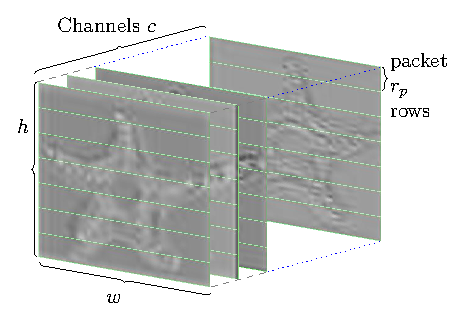
\includegraphics[scale=0.9]{tensorlostviz3icip.pdf}
		\caption{Tensor from layer add\_1 of ResNet-18. Several consecutive rows in each channel form a feature data packet.}
	\end{figure}
\end{frame}

\begin{frame}
	\frametitle{Corrupted tensor visualization}
	\begin{figure}
		\begin{minipage}{.48\textwidth}
			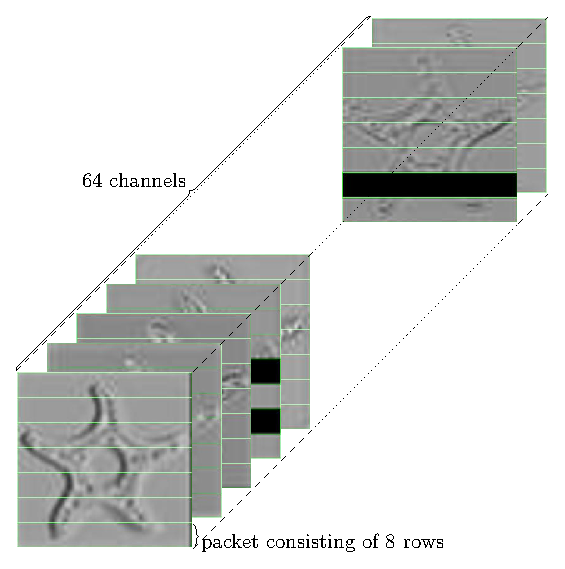
\includegraphics[width=0.9\linewidth]{tensorviz4.pdf}
			\caption{Corrupted ResNet-18 deep feature tensor consisting of 64 channels. Each channel consists of 7 packets. Packets are $8 \times 56$ blocks of deep feature tensor values.}
		\end{minipage}\hfill
		\begin{minipage}{.48\textwidth}
			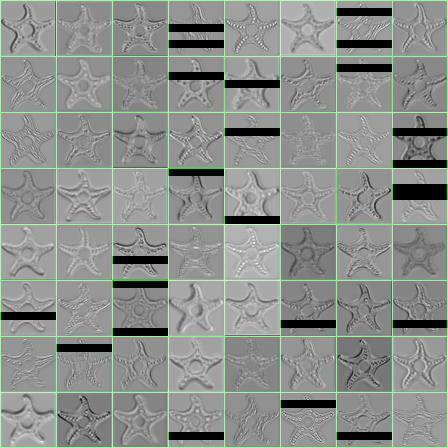
\includegraphics[width=0.9\linewidth]{tiledgridtensor.jpg}
			\caption{Tiled tensor $\tilde{\mathcal{X}} \in \mathbb{R}^{56 \times 56 \times 64}$ visualization. Each tile represents a channel of shape $56 \times 56$. }
		\end{minipage}
	\end{figure}
\end{frame}



\section{Proposed method}

\section{Experiments}
\subsection{Visual results}

\begin{frame}
    \frametitle{Visual results}
\end{frame}


\subsection{Monte Carlo experiments}

\begin{frame}
\frametitle{Monte Carlo experiments}
\end{frame}

\section{Conclusions}
\begin{frame}
	\frametitle{Conclusions and recommendations}
	\begin{itemize}
		\item CALTeC exploits intra- and inter-channel similarity in deep feature tensors to find the best candidates in other channels to fill the gaps in corrupted packetized deep feature tensors.
		\item CALTeC adjusts the recovered data with an affine transformation.
		\item CALTeC is slower than ALTeC but unlike ALTeC, it does not require pre-training.
		\item Both ALTeC and CALTeC are much faster than SiLRTC and HaLRTC.
		\item Future work can focus on extending DFTS to run different tasks and to incorporate different compression methods for the transmitted deep feature tensor.
	\end{itemize}
\end{frame}

%------------------------------------------------
\section{Implementation}
\begin{frame}
\frametitle{Implementation \& Results}
Public repository for DFTS2: \url{https://github.com/AshivDhondea/DFTS_TF2}.

This repository also contains the packet loss traces and Monte Carlo experiment results presented in this paper.
	\end{frame}
	
%---------------------------------------------
\section{References}
\bibliographystyle{ieeetr}
\bibliography{icipcaltecrefs}
%-----------------------------------------------
\end{document} 